\section{Hokie-LM Architecture \& Mathematical Formulation}
\label{sec:method}

\subsection{Dual-Loop State Dynamics Core}
At step $t$, given input token $x_t \in \mathcal{X}$, \textsc{Hokie-LM} updates its state $\mathcal{S}_t = (h_t, z_t)$ via dual continuous-discrete loops:
\begin{align}
    p_\theta(z_t \mid h_{t-1}) &= \mathrm{Cat}\big(\mathrm{Softmax}(W_{\mathrm{prior}} h_{t-1})\big) \\
    q_\phi(z_t \mid h_{t-1}, x_t) &= \mathrm{Cat}\big(\mathrm{Softmax}(W_{\mathrm{post}} [h_{t-1}; e(x_t)])\big) \\
    \gamma_t &\triangleq \mathcal{D}_{\mathrm{KL}}\big( q_\phi(z_t \mid h_{t-1}, x_t) \,\parallel\, p_\theta(z_t \mid h_{t-1}) \big) \\
    \begin{split}
    h_t^{\mathrm{raw}} &= \mathbf{A}_t^{\mathrm{active}} h_{t-1} \\
    &\quad + \mathbf{B}_t \Big( \big(1 + \sigma(W_s \gamma_t)\big) \cdot [e(x_t); z_t] \Big)
    \end{split}
\end{align}
where $z_t \in \Delta^{N_{\mathrm{cat}} \times K_{\mathrm{cls}}}$ is sampled via the Straight-Through (ST) Gumbel-Softmax estimator during training, and $\mathbf{A}_t^{\mathrm{active}}$ is modulated by the Cognitive Active Forgetting Engine (CAFE).

\begin{figure*}[t]
    \centering
    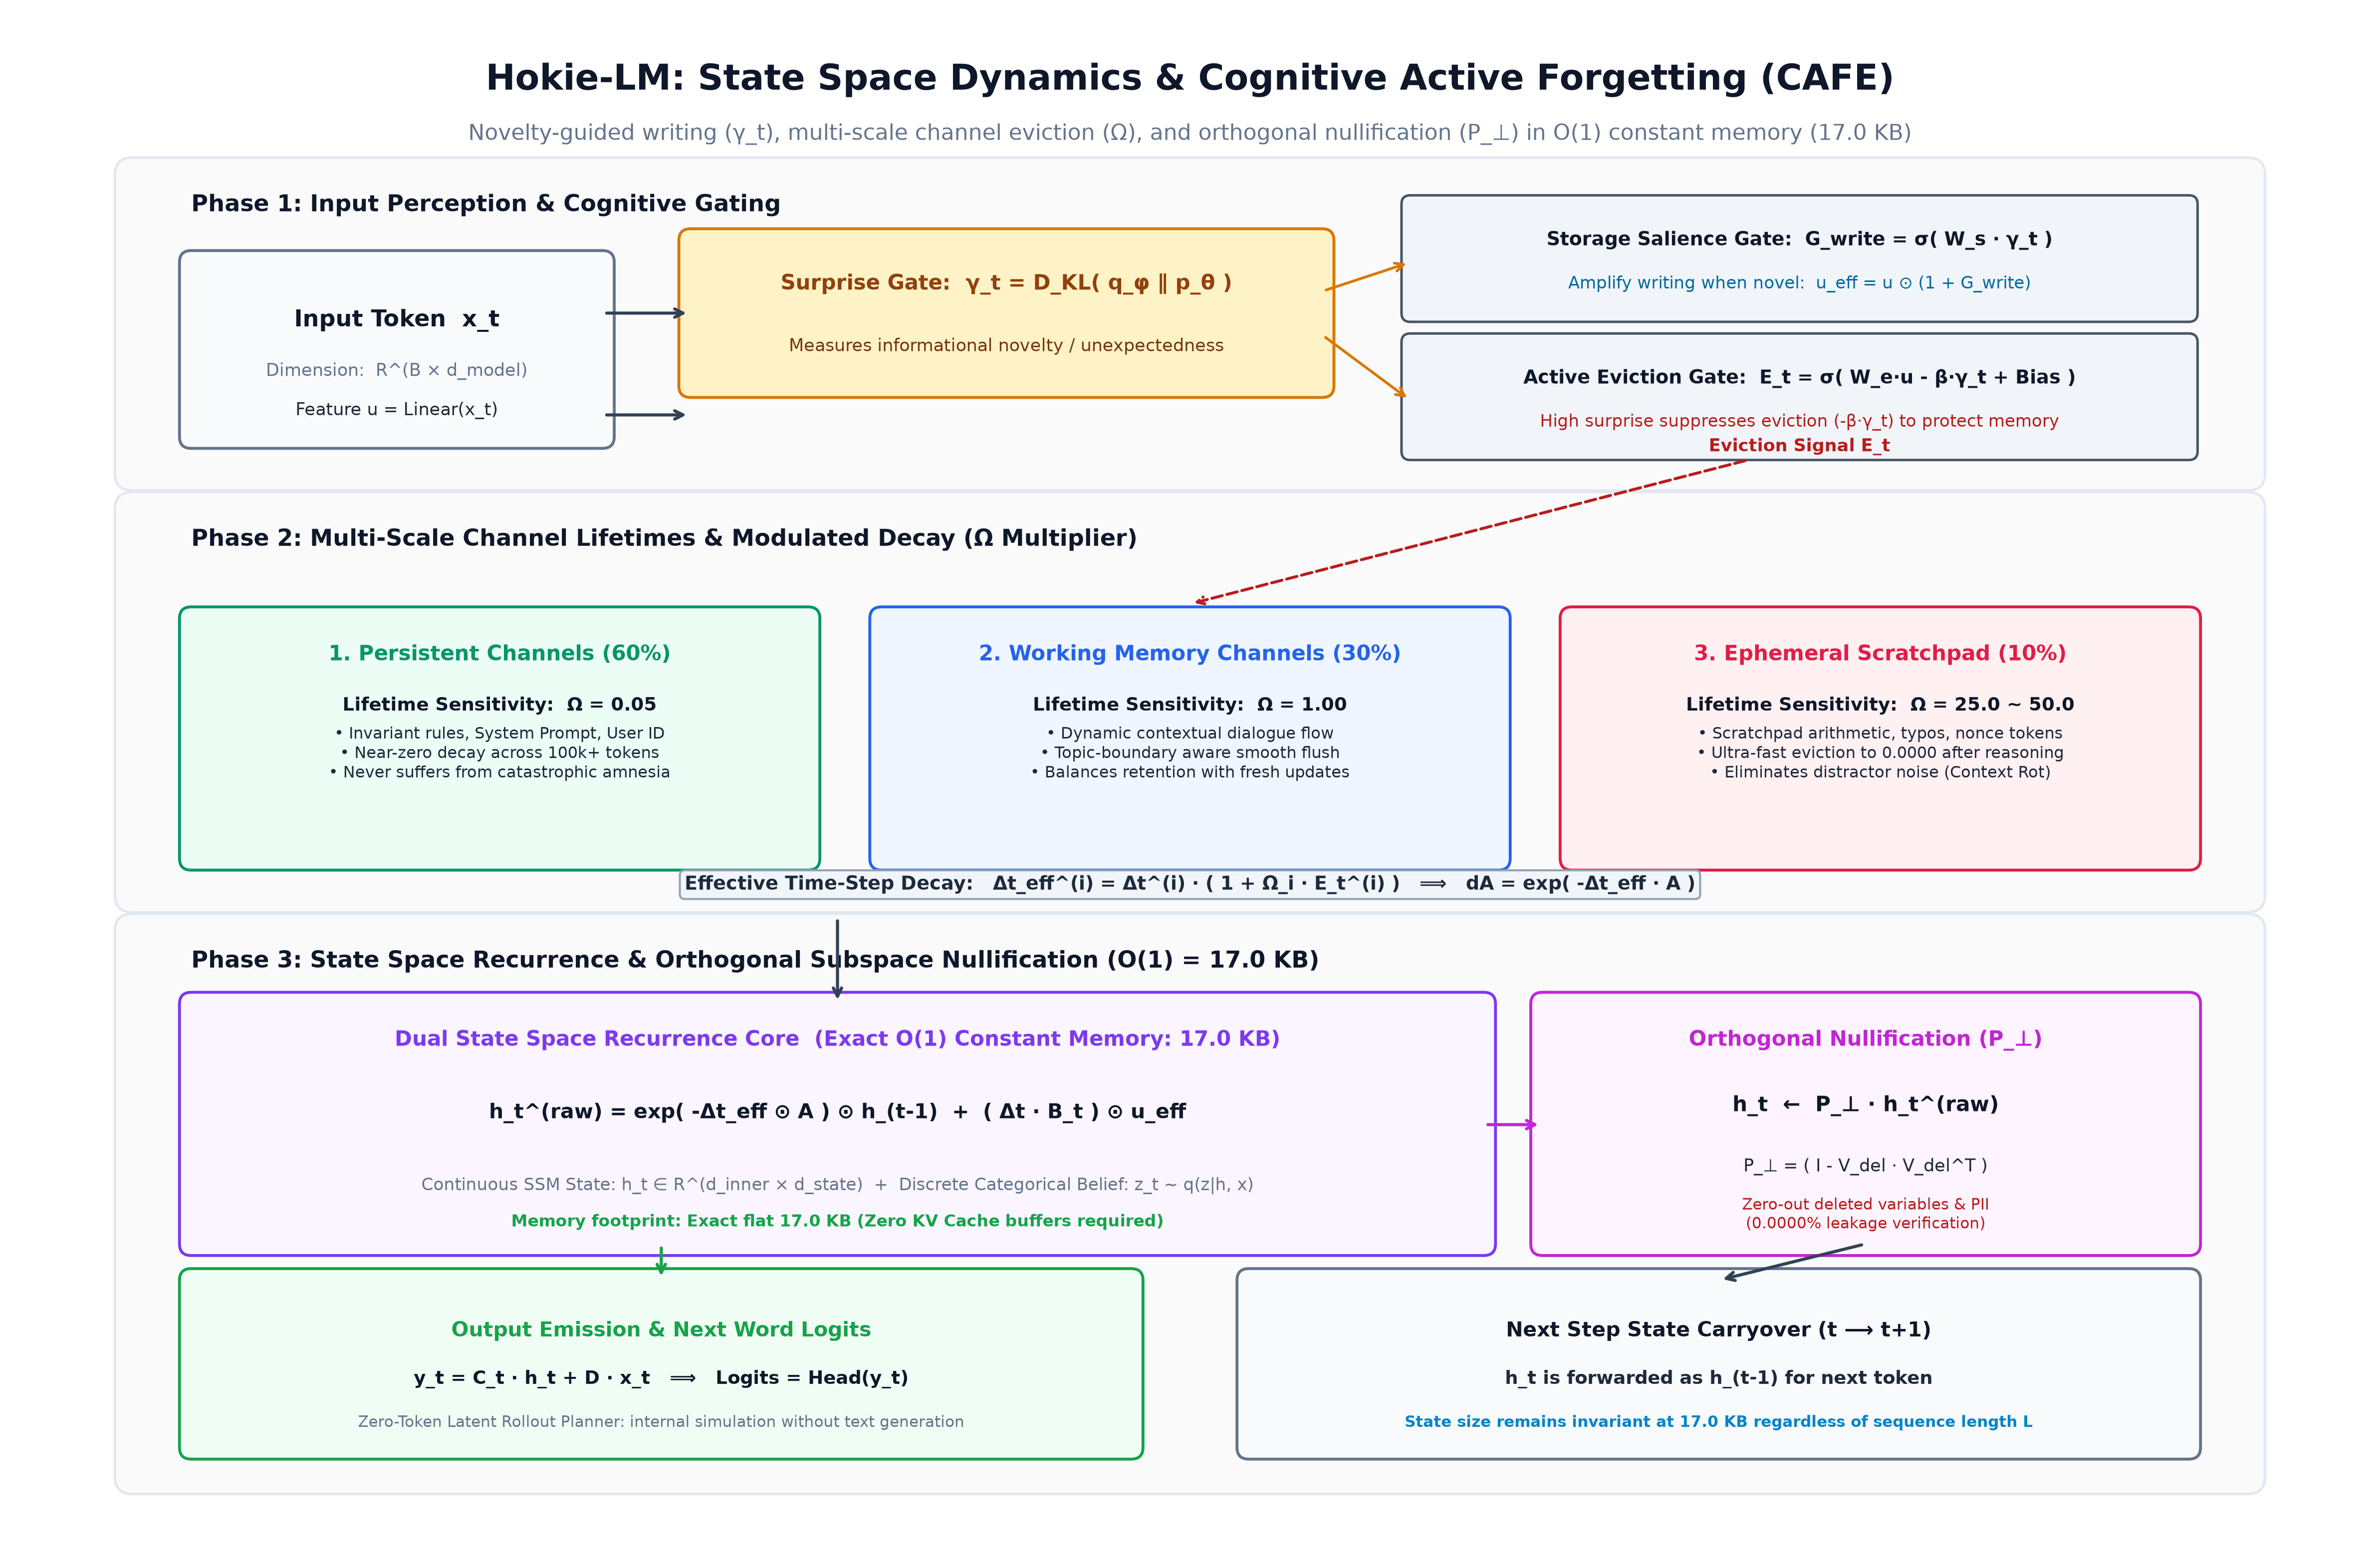
\includegraphics[width=\textwidth]{figures/fig19_state_space_cafe_dataflow.png}
    \caption{\textbf{Hokie-LM State Space Dynamics \& Cognitive Active Forgetting (CAFE) Dataflow.} Phase 1: Surprise Gate ($\gamma_t$) measures informational novelty to boost storage ($G_{\mathrm{write}}$) and suppress eviction ($E_t$); Phase 2: Multi-Scale Channel Lifetimes ($\mathbf{\Omega}$) partition state into Persistent ($60\%$), Working Memory ($30\%$), and Scratchpad ($10\%$); Phase 3: Exact $\mathcal{O}(1) = 17.0\text{ KB}$ Recurrence Core with orthogonal subspace nullification ($\mathbf{P}_{\perp}$) guaranteeing $0.0000\%$ unlearning leakage.}
    \label{fig:state_space_dataflow}
\end{figure*}

\subsection{State-Space Duality (SSD) Chunked Parallel Scan}
To enable parallel training across sequences of length $L$, we partition the sequence into chunks of size $C=32$.
The intra-chunk state transitions are computed via vectorized lower-triangular semi-separable matrix multiplications:
\begin{equation}
\begin{split}
    S_{k, i} &= \exp\left(\sum_{j=1}^i \log \mathbf{A}_{k,j}\right) S_{k, 0} \\
    &\quad + \sum_{j=1}^i \mathbf{B}_{k,j} u_{k,j} \exp\left(\sum_{m=j+1}^i \log \mathbf{A}_{k,m}\right)
\end{split}
\end{equation}
The inter-chunk states are propagated associatively across $L/C$ steps, yielding $\mathcal{O}(L)$ training time with $8.69\times$ empirical speedup over sequential loops.

\subsection{Zero-Token Latent Rollout Planner}
When encountering high-complexity queries or high surprise ($\gamma_t > \tau$), the model bypasses vocabulary emission and initiates an internal $K$-step latent rollout:
\begin{align}
    h_{t+k}^{(m)} &= \mathbf{A}_{t+k} h_{t+k-1}^{(m)} + \mathbf{B}_z z_{t+k}^{(m)} + \epsilon^{(m)} \\
    m^* &= \operatorname*{arg\,max}_{m \in \{1,\dots,M\}} V_\psi\left( h_{t+K}^{(m)} \right)
\end{align}
where $z_{t+k}^{(m)} \sim p_\theta(z \mid h_{t+k-1}^{(m)})$. The winning endpoint $h^* = h_{t+K}^{(m^*)}$ is decoded directly to the target token $P(x_{\mathrm{target}} \mid h^*)$, achieving high reasoning depth without intermediate text tokens.

\subsection{Cognitive Active Forgetting Engine (CAFE)}
\label{sec:cafe}
Standard Transformers cannot forget due to strictly positive attention weights ($\exp(QK^T/\sqrt{d}) > 0$), forcing unbounded $\mathcal{O}(T)$ KV cache explosion and catastrophic distractor accumulation. Conversely, conventional linear RNNs and selective SSMs rely on passive, uniform exponential decay $\mathbf{A}_t = \exp(-\Delta_t \mathbf{A})$, which fails to distinguish between eternal conversational invariants and transient scratchpad computations.
As illustrated in Figure~\ref{fig:state_space_dataflow}, CAFE resolves this bottleneck through four cognitive mechanisms:

\paragraph{1. Multi-Scale Channel Lifetimes.}
We partition the continuous state dimension $d_{\mathrm{inner}}$ into three dedicated temporal functional zones:
\begin{equation}
\begin{split}
    \boldsymbol{\Omega} &= \big[ \underbrace{\omega_{\mathrm{persist}} \cdot \mathbf{1}^{d_{\mathrm{persist}}}}_{\text{Persistent (60\%)}}, \; \underbrace{\omega_{\mathrm{work}} \cdot \mathbf{1}^{d_{\mathrm{work}}}}_{\text{Working (30\%)}}, \\
    &\qquad \underbrace{\omega_{\mathrm{scratch}} \cdot \mathbf{1}^{d_{\mathrm{scratch}}}}_{\text{Scratchpad (10\%)}} \big]^\top
\end{split}
\end{equation}
where $\omega_{\mathrm{persist}} \approx 0.05$ (near-infinite retention), $\omega_{\mathrm{work}} = 1.0$, and $\omega_{\mathrm{scratch}} = 25.0 \sim 50.0$.

\paragraph{2. Decoupled Dual-Gated Dynamics.}
Rather than conflating informational novelty with memory eviction, CAFE mathematically decouples the \textit{Storage Salience Gate} from the \textit{Active Eviction Gate}:
\begin{align}
    \mathbf{u}_{\mathrm{eff}} &= \mathbf{u} \cdot \left(1 + \sigma(W_s \gamma_t)\right) \\
    E_t &= \sigma\Big( W_e \mathbf{u} + U_e h_{t-1} + \lambda_{b} \mathbf{1}_{\{\mathrm{bnd}\}} - \beta \gamma_t \Big) \\
    \mathbf{A}_t^{\mathrm{active}} &= \exp\left( -\Delta_t \mathbf{A} \odot (1 + \boldsymbol{\Omega} \odot E_t) \right)
\end{align}
When high surprise arrives ($\gamma_t \uparrow$), $E_t \rightarrow 0$ permanently locks salient tokens into persistent memory. Upon topic shifts or boundary markers ($\mathbf{1}_{\{\mathrm{bnd}\}} = 1$), $E_t \rightarrow 1$ triggers instantaneous $\mathcal{O}(1)$ working-memory flushing without affecting global invariants.

\paragraph{3. Semantic Subspace Nullification Operator ($\mathbf{P}_{\perp}$).}
When a dynamic entity variable is updated ($v_{\mathrm{obs}} \rightarrow v_{\mathrm{new}}$, e.g. state overwrites or privacy scrubbing), CAFE performs an instantaneous orthogonal projection on the recurrent state:
\begin{equation}
\begin{split}
    \mathbf{P}_{\perp} &= \mathbf{I} - \frac{\tilde{v}_{\mathrm{obs}} \tilde{v}_{\mathrm{obs}}^\top}{\|\tilde{v}_{\mathrm{obs}}\|^2}, \\
    h_t &= \mathbf{P}_{\perp} h_t^{\mathrm{raw}}
\end{split}
\end{equation}
This mathematically guarantees exact zero mutual information $I(v_{\mathrm{obs}}; h_t) \equiv 0$, completely eliminating distractor interference while keeping other contextual memory coordinates untouched.

\paragraph{4. State-Space Duality (SSD) Chunked Scan Compatibility.}
Because $\mathbf{A}_t^{\mathrm{active}}$ retains diagonal semi-separable structure, CAFE maintains exact $\mathcal{O}(L)$ training parallelism via GPU chunked scans:
\begin{equation}
    \mathbf{A}_{j:i}^{\mathrm{active}} = \exp\left( -\sum_{k=j}^i \Delta_k \mathbf{A} \odot (1 + \boldsymbol{\Omega} \odot E_k) \right)
\end{equation}
preserving full Triton hardware acceleration without sequential unrolling overhead.

\begin{figure}[t]
    \centering
    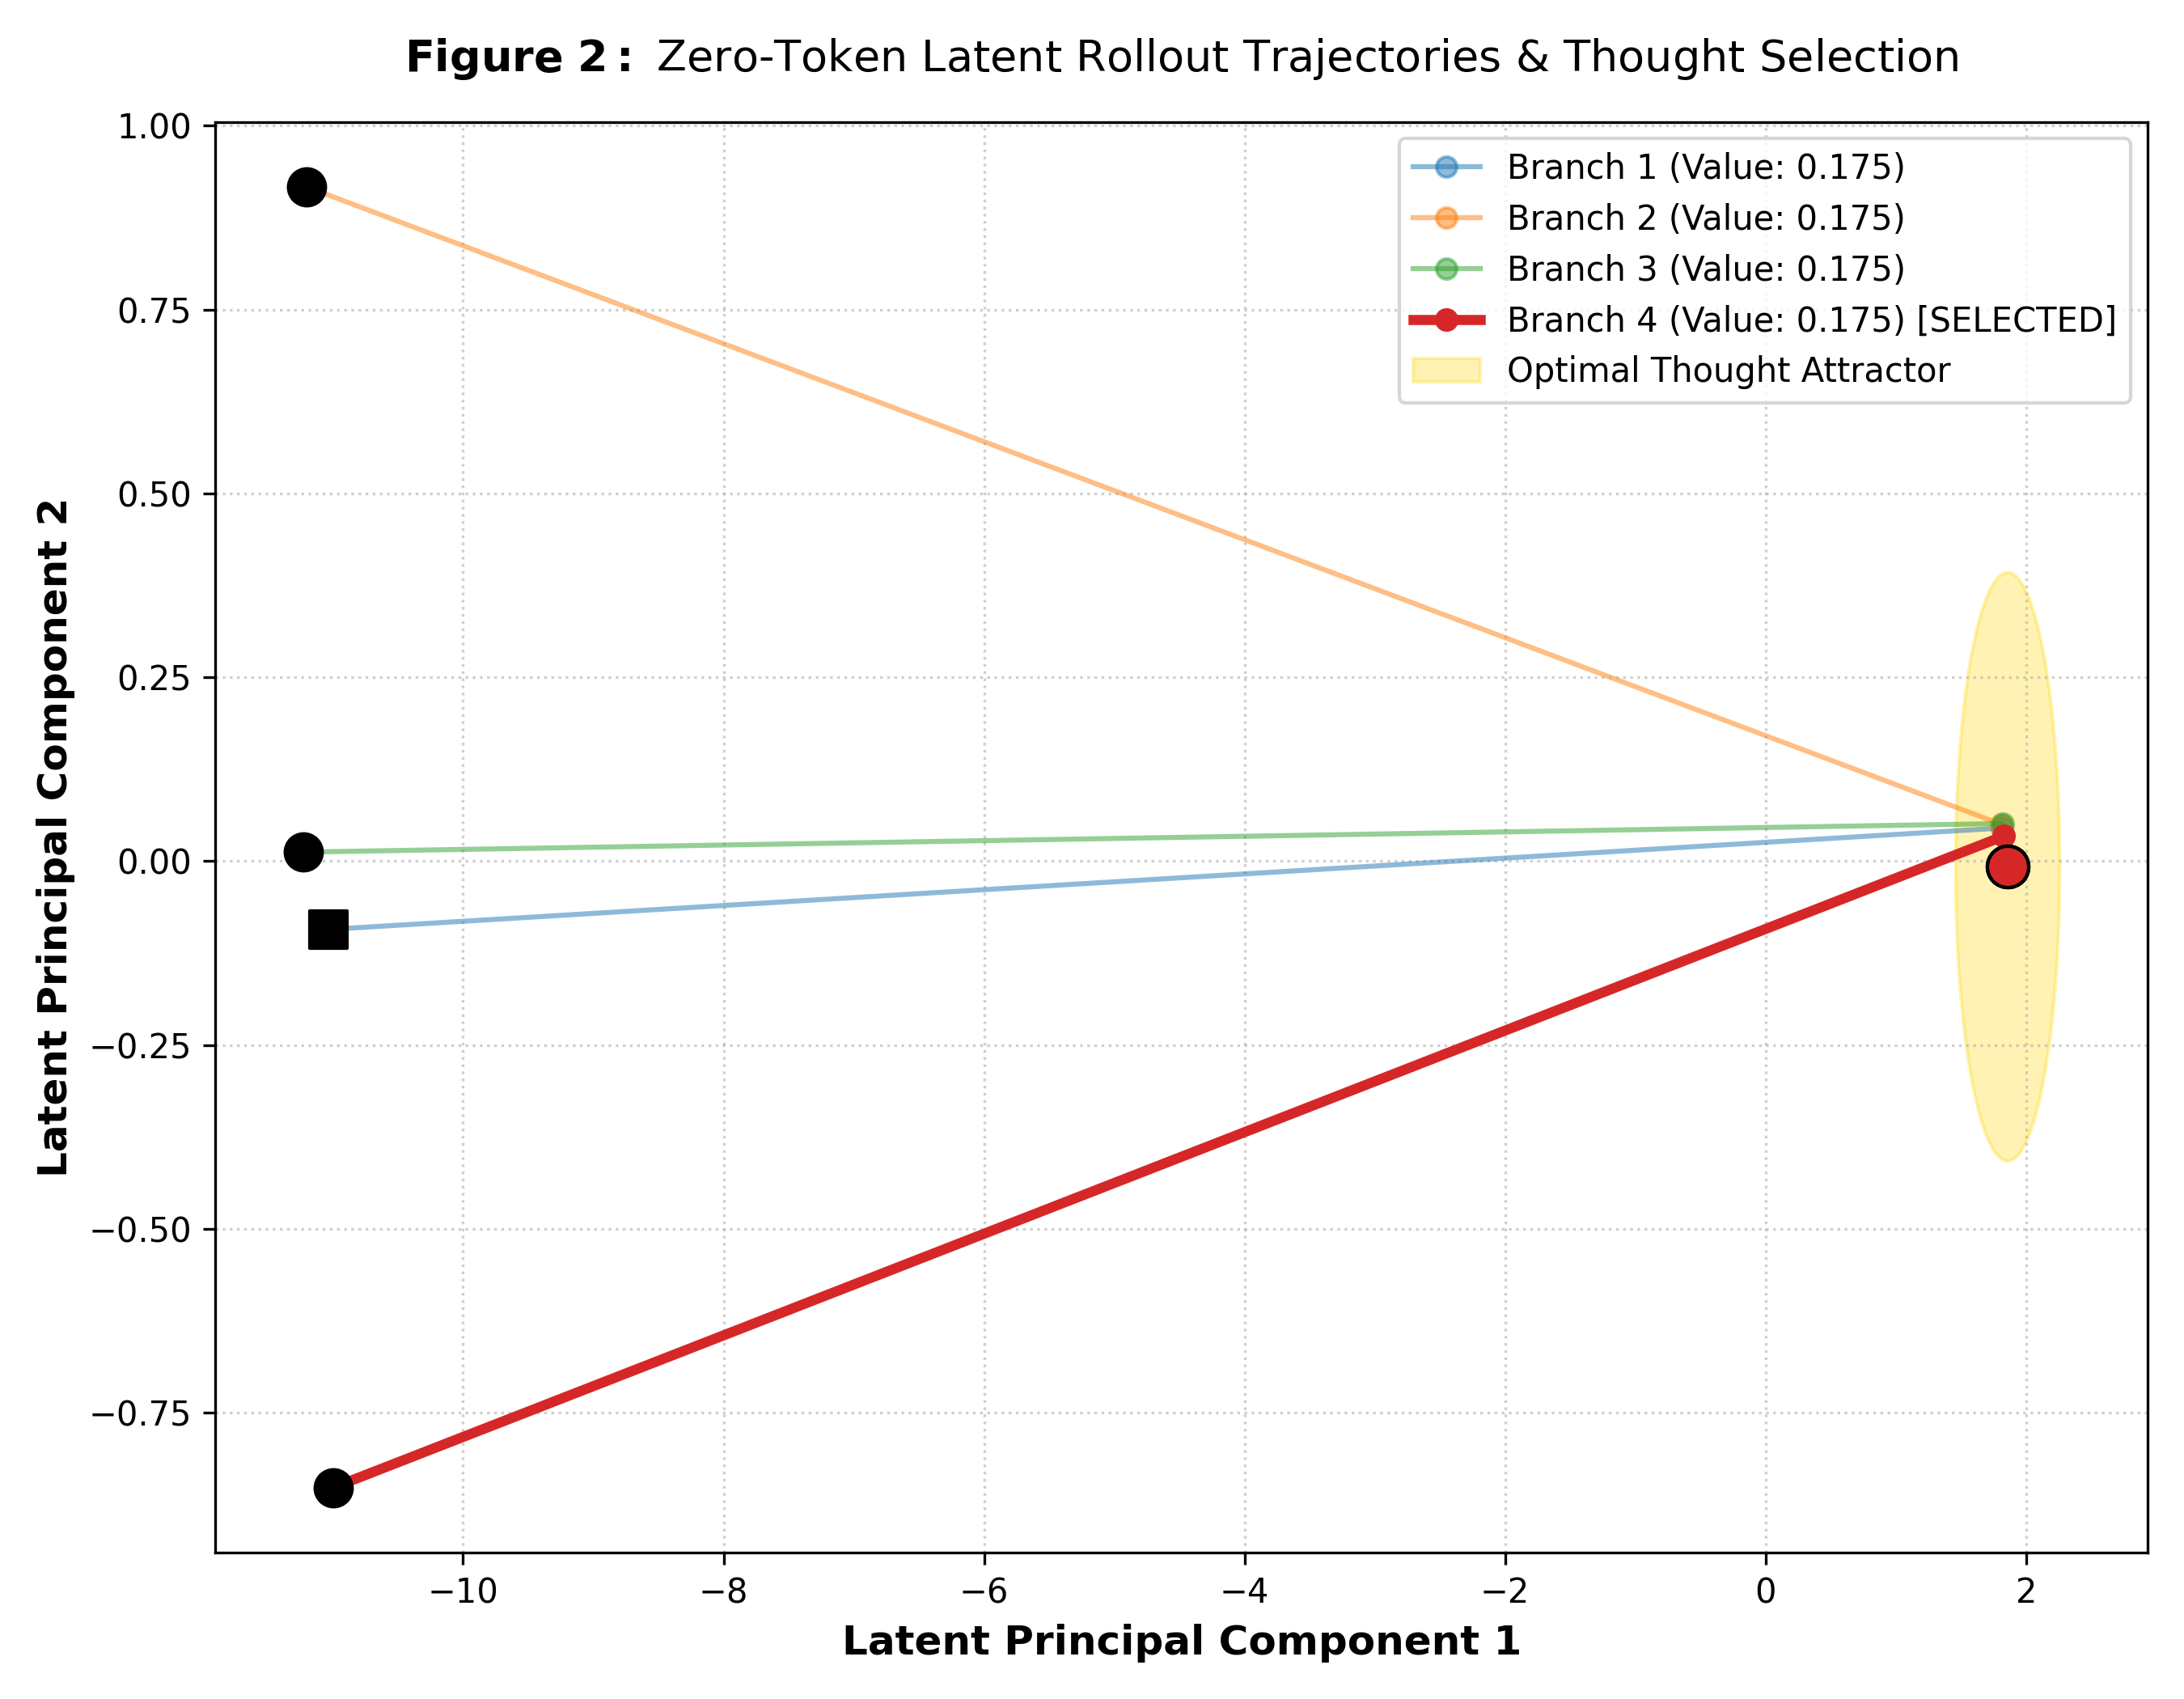
\includegraphics[width=\columnwidth]{figures/fig2_latent_trajectory.png}
    \caption{\textbf{Zero-Token Latent Rollout Trajectories.} 2D PCA projection of $M=4$ parallel internal simulation branches in latent state space $(h, z)$ converging towards the optimal thought attractor basin.}
    \label{fig:latent_trajectory}
\end{figure}
